
 \documentclass[a4paper,12pt]{article} % This defines the style of your paper

% We usually use the article type. The additional parameters are the format of the paper you want to print it on and the standard font size. For us this is a4paper and 12pt.

%%%%%%%%%%%%%%%%%%%%%%%%%%%%%%%%%%%%%%%%%%%%%%%%
% 2. Packages
%%%%%%%%%%%%%%%%%%%%%%%%%%%%%%%%%%%%%%%%%%%%%%%%

% Packages are libraries of commands that LaTeX can call when compiling the document. With the specialized commands you can customize the formatting of your document.
% If the packages we call are not installed yet, TeXworks will ask you to install the necessary packages while compiling.

% First, we usually want to set the margins of our document. For this we use the package geometry. We call the package with the \usepackage command. The package goes in the {}, the parameters again go into the [].
\usepackage[top = 2.5cm, bottom = 2.5cm, left = 2.5cm, right = 2.5cm]{geometry} 
\usepackage{pagecolor,lipsum}
\pagecolor{white}
\usepackage{float}
\usepackage{listings}

% Unfortunately, LaTeX has a hard time interpreting German Umlaute. The following two lines and packages should help. If it doesn't work for you please let me know.
\usepackage[T1]{fontenc}
\usepackage[utf8]{inputenc}


% The following two packages - multirow and booktabs - are needed to create nice looking tables.
\usepackage{multirow} % Multirow is for tables with multiple rows within one cell.
\usepackage{booktabs} % For even nicer tables.

% As we usually want to include some plots (.pdf files) we need a package for that.
\usepackage{graphicx} 

% The default setting of LaTeX is to indent new paragraphs. This is useful for articles. But not really nice for homework problem sets. The following command sets the indent to 0.
\usepackage{setspace}
\setlength{\parindent}{0in}

% Package to place figures where you want them.
\usepackage{float}

% The fancyhdr package let's us create nice headers.
\usepackage{fancyhdr}


%%%%%%%%%%%%%%%%%%%%%%%%%%%%%%%%%%%%%%%%%%%%%%%%
% 3. Header (and Footer)
%%%%%%%%%%%%%%%%%%%%%%%%%%%%%%%%%%%%%%%%%%%%%%%%

% To make our document nice we want a header and number the pages in the footer.

\pagestyle{fancy} % With this command we can customize the header style.

\fancyhf{} % This makes sure we do not have other information in our header or footer.

% Similar commands work for the footer (\lfoot, \cfoot and \rfoot).
% We want to put our page number in the center.
\cfoot{\footnotesize \thepage} 


%%%%%%%%%%%%%%%%%%%%%%%%%%%%%%%%%%%%%%%%%%%%%%%%
% 4. Your document
%%%%%%%%%%%%%%%%%%%%%%%%%%%%%%%%%%%%%%%%%%%%%%%%

% Now, you need to tell LaTeX where your document starts. We do this with the \begin{document} command.
% Like brackets every \begin{} command needs a corresponding \end{} command. We come back to this later.

\begin{document}


%%%%%%%%%%%%%%%%%%%%%%%%%%%%%%%%%%%%%%%%%%%%%%%%
%%%%%%%%%%%%%%%%%%%%%%%%%%%%%%%%%%%%%%%%%%%%%%%%

%%%%%%%%%%%%%%%%%%%%%%%%%%%%%%%%%%%%%%%%%%%%%%%%
% Title section of the document
%%%%%%%%%%%%%%%%%%%%%%%%%%%%%%%%%%%%%%%%%%%%%%%%

% For the title section we want to reproduce the title section of the Problem Set and add your names.

\thispagestyle{empty} % This command disables the header on the first page. 

\begin{tabular}{p{15.5cm}} % This is a simple tabular environment to align your text nicely 
\begin{center}
\small $^1$University of Florence, $^2$University of Prague, $^3$University of Bergamo, $^4$Istat\\
\end{center}
\end{tabular} % Our tabular environment ends here.
\vspace*{0.3cm} % Now we want to add some vertical space in between the line and our title.

\begin{center} % Everything within the center environment is centered.
	{\Large \bf Graph Analysis of International Trading Network} % <---- Don't forget to put in the right number
	\vspace{6mm}
	
        	\textbf{\small Main Author}\\
	{\small Fabbrico Davide$^1$, Khateeb Ahmad Arsalan$^2$ and Pagnoncelli Diego$^3$}\\
	\vspace{3mm}
	\textbf{\small Istat Reference Tutor}\\
	{\small Bruno Mauro$^4$, Causo Maria Serena$^4$ and De Fausti Fabrizio$^4$}\\
	
		
\end{center}  

\vspace{0.5cm}
{\small \textbf{Keywords} Graph Analysis, Plotting, Regression, International Trade, Geography, Fuel consumption, Greeness.}

\section{Abstract}

In our analysis we are interested in the graph analysis of the International trading network between 2019 and 2021. 
To compute our analysis we exploited the “Comext Data”. In particular our data are Transport HS and Transport NSTR.
We also made use of data about distances among countries which was generated by using QGIS software which was provided by our reference tutor, De Fausti Fabrizio. 
In order to better understand the commercial connection we decided to create an index which tells us how several means of transportation affects pollution in different places in the world throughout the year. The name of our index is “Greeness”. To compute the index, we started from the dependent variable which is “pollution” that is define as follows: fuel (fuel used per kilometers run), mean of transport (we created a dummy variable that contains: 'Road', 'Air', 'Post', 'Sea', ‘Rail’), type of product traded, distance  (km run) and the error term. 
We analyze two type of \textbf{Greeness}, a local metric and a global metric.
One other motivation why we \\

From an early analysis, we have found that: 
\newpage
Our main function takes as input a set of data (dataframe), the month and year of interest for the analysis, the product involved, the type of flow (import or export), type of transport (Rail, Air, Road, etc...) and a threshold to control the percentage of imports/exports within the analysis, in particular the user can choose to manage euros or quantities in kilograms. This function filters the data set for each user choice through the appropriate forms and returns a direct graph with the previously desired filters. The graph G, which represents an instance for each product traded, represented below (Figure 1) is a doublet $(V, E)$ in which $V$ is the set of nodes which represent each country and $E$ is the set of edges that connect two countries if an exchange has taken place between them. The edges also contain weights which indicate the distance between the two connected countries. The data have been aggregated, that is, if we have two imports from Italy to the Czech Republic, always under the assumption of the same product and the same period, these two imports will be added in the quantity of kilograms and the quantity of euros. After we have the data relating to the fuel consumption for each vehicle, we can calculate how many liters of fuel it has consumed and consequently the level of pollution for each transport. Once the liters of fuel have been calculated, the nodes corresponding to each country will have another attribute called \textbf{Total Liter}. This measure will be calculated as the sum of the weights (which will subsequently become liters of fuel and no longer distances) of the edges exiting the node (out-degree).\\

\begin{figure}[H]
	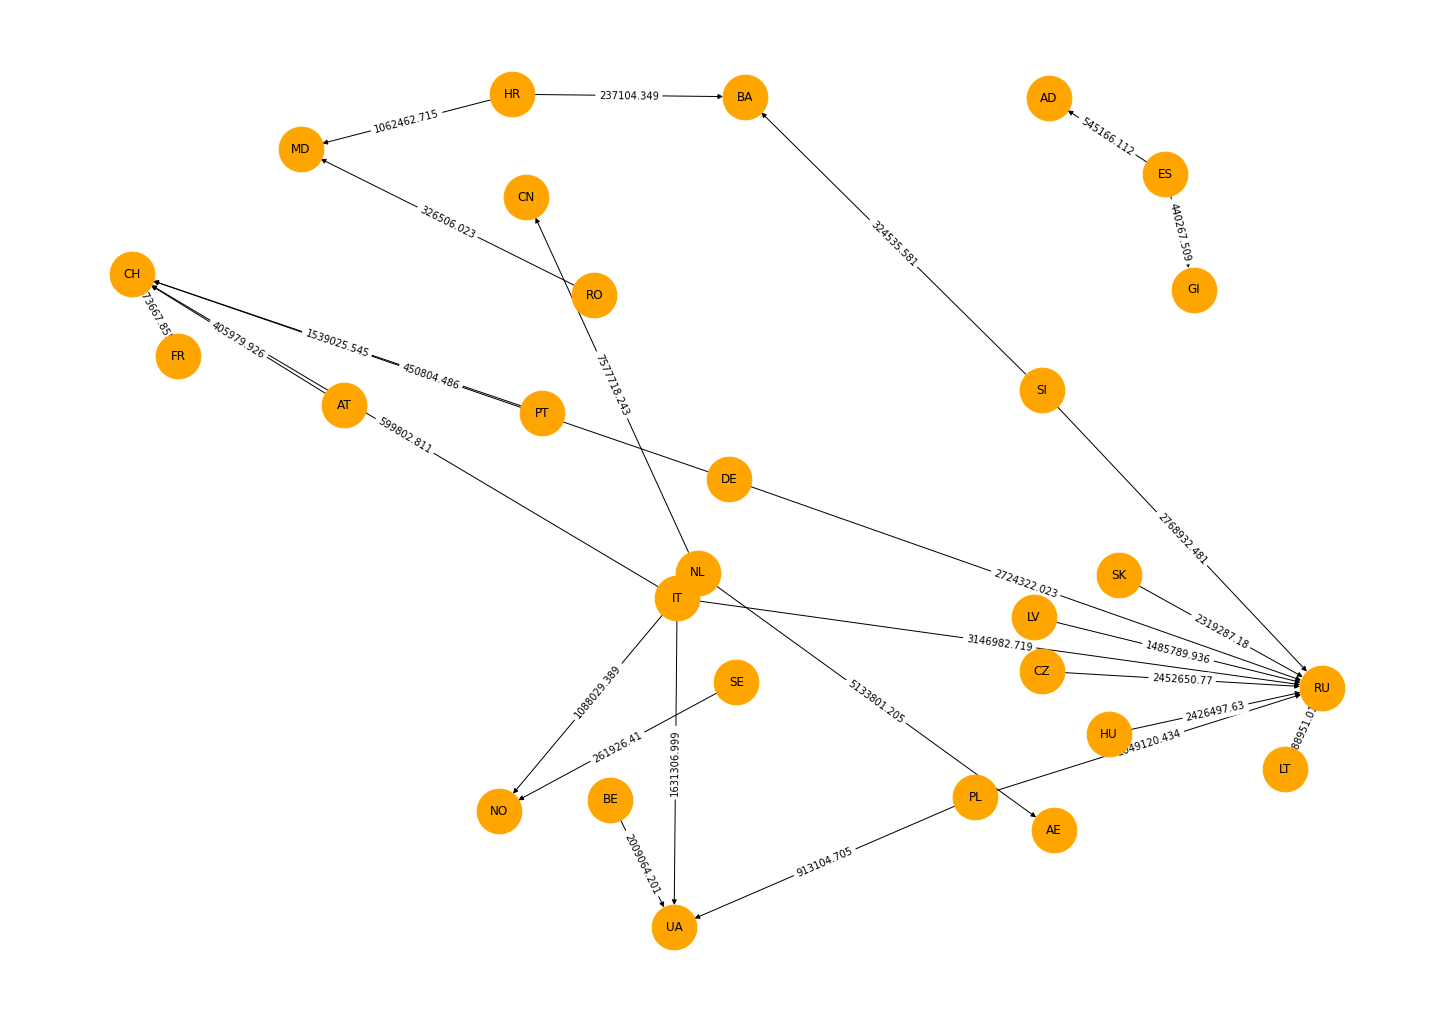
\includegraphics[height=10.3cm, width=14cm]{graph}
	\caption{Graph relating to the export via Road of 20 percent of the flow of product number 220110 of the period October 2019, ordering by quantity of euros.}   
 	 \label{fig:picture}
\end{figure}


\end{document}
